\documentclass{article}
\usepackage[utf8]{inputenc}

\title{Chem132A: Lecture 05}
\author{Shane Flynn (swflynn@uci.edu) }
\date{10/9/17}


\usepackage{graphicx}
\usepackage{amsmath}
\usepackage{braket}
\usepackage[margin=0.7in]{geometry}
\usepackage{hyperref}


\newcommand{\be}{\begin{equation}}
\newcommand{\ee}{\end{equation}}
\newcommand{\benum}{\begin{enumerate}}
\newcommand{\eenum}{\end{enumerate}}
\newcommand{\pd}{\partial}

\begin{document}

\maketitle

\section*{The Newest State Function: Entropy}
Entropy has been introduced in previous courses as the amount of 'disorder'. 
In this course we will define the Entropy in terms of a reversible process. 
\be
S \equiv \frac{q_r}{T}
\ee

We are not going to prove it, however, Entropy is a state function, which means we can write
\be
\Delta S = \int_i^f \frac{\delta q_r}{T}
\ee

To show that this definition of Entropy is a state function is actually a difficult exercise using differential equations. 
If you are interested, it can be done using an \textbf{Integrating Factor}.

The First Law of Thermodynamics looks at the transfer of energy in terms of work and heat. 
The Second Law of Thermodynamics is interested in the spontaneity of a process. 

There are various (equivalent) ways of stating Second Law such as:
\benum
\item Heat does not flow spontaneously from a cold body to a hotter body.
\item No process is possible in which the sole result is the absorption of heat from a reservoir and its complete conversion into work.
\item The Entropy of an isolated system increases in the course of a spontaneous change ($\Delta$S$_{\text{total}} >$ 0)
\eenum

A more fundamental definition of the Entropy can be explored through \textbf{Statistical Mechanics}. 
Boltzmann is well know for his famous formula (engraved on his tombstone) 
\be
S = k \ln W
\ee
This definition is in terms of the microstates available to a system (W). 
A microstate essentially refers to any of the possible physical states available to the system (think of all the different ways the atoms can be arranged).
It is important to note that this equation is in terms of the actual Entropy itself, and not the change in Entropy.

Intuitively we can think of entropy as disorder, and we know from experience (think of how easily your room becomes a mess) that life seems to favor generating more disorder (higher Entropic States).


We need to be careful about context when discussing changes in Entropy. 
The Second Law puts a constraint on the Entropy generation of the Entire Universe. 
This constraint is non-negotiable, if the Entropy of your system decreases in an irreversible processes, the Entropy of the surroundings (the universe) will increase. 

\section*{Phase Changes}
It turns out that a change of phase at the phase transition temperature is a reversible process. 

\be
\Delta_{\text{trs}} = \frac{q_r}{T_{\text{trs}}}
\ee
If we have a constant pressure than the heat and the Enthalpy are related and we can write
\be
\Delta_{\text{trs}} = \frac{\Delta_{\text{trs}}H}{T_{\text{trs}}}
\ee

Here temperature must be positive (Kelvin scale) therefore the sign of Enthalpy directly determines the sign of the Entropy. 
Intuition would tell us that melting a substance requires heat, and we would guess that the entropy of transition would therefore be positive.

Consider how the Entropy change upon heating your system. 
\be
\begin{split}
\Delta S &= \int_i^f \frac{\delta q_r}{T} \\
S_f - S_i &= \int_i^f \frac{\delta q_r}{T} \\
S(T_f) &= S(T_i) + \int_{T_i}^{T_f} \frac{\delta q_r}{T} = S(T_i) + \int_{T_i}^{T_f} \frac{C_P(T)dT}{T} \\
S(T_f) &= S(T_i) + C_p \ln\frac{T_f}{T_i}
\end{split}
\ee

We can generate a simple equation for calculating the change in Entropy assuming a heat capacity that is not a function of temperature and integrating over our temperature range (assuming constant P and only PV work). 

Practically speaking; calculations that go through a phase transition need to be broken into heating the sample, and then performing the physical phase transition. 
Also note, the heat capacity of one physical state is not the same as that of another physical state.
This must be accounted for while performing Entropy calculations using the above method. 

\section*{The Third Law of Thermodynamics}
The Third Law of Thermodynamics states: The Entropy of all perfect crystalline substances is 0 at T=0(K). 

If you do not have a perfect crystal a \textbf{Residual Entropy} which is non-zero can occur.
This means that at 0K there are multiple configurations (microstates) all with the same energy, and therefore contribute to the Boltzmann Entropy Equation. 

When thinking about the Laws of Thermodynamics, remember that the First Law discusses the energetics of a system, and the Second Law discusses the spontaneity of a process. 

\section*{Supplemental; The Carnot Cycle}
The Carnot Cycle describes a very famous engine used to illustrate the concept of efficiency. 
It was also introduced to illustrate Entropy may in-fact be a state function. 

We know from the first law that U = Q + W, and we know that our state functions must be 0 over a closed cycle $\oint ds = 0$, $\oint dU = 0$, $\oint \delta q \neq 0$, $\oint \delta w \neq 0$.
So we should confirm that Internal Energy and Entropy are 0 over 1 cycle of the engine.
To do this we will need to determine the heat/work associated with each of the four steps in the Carnot Cycle.

\begin{figure}[h]
    \centering
    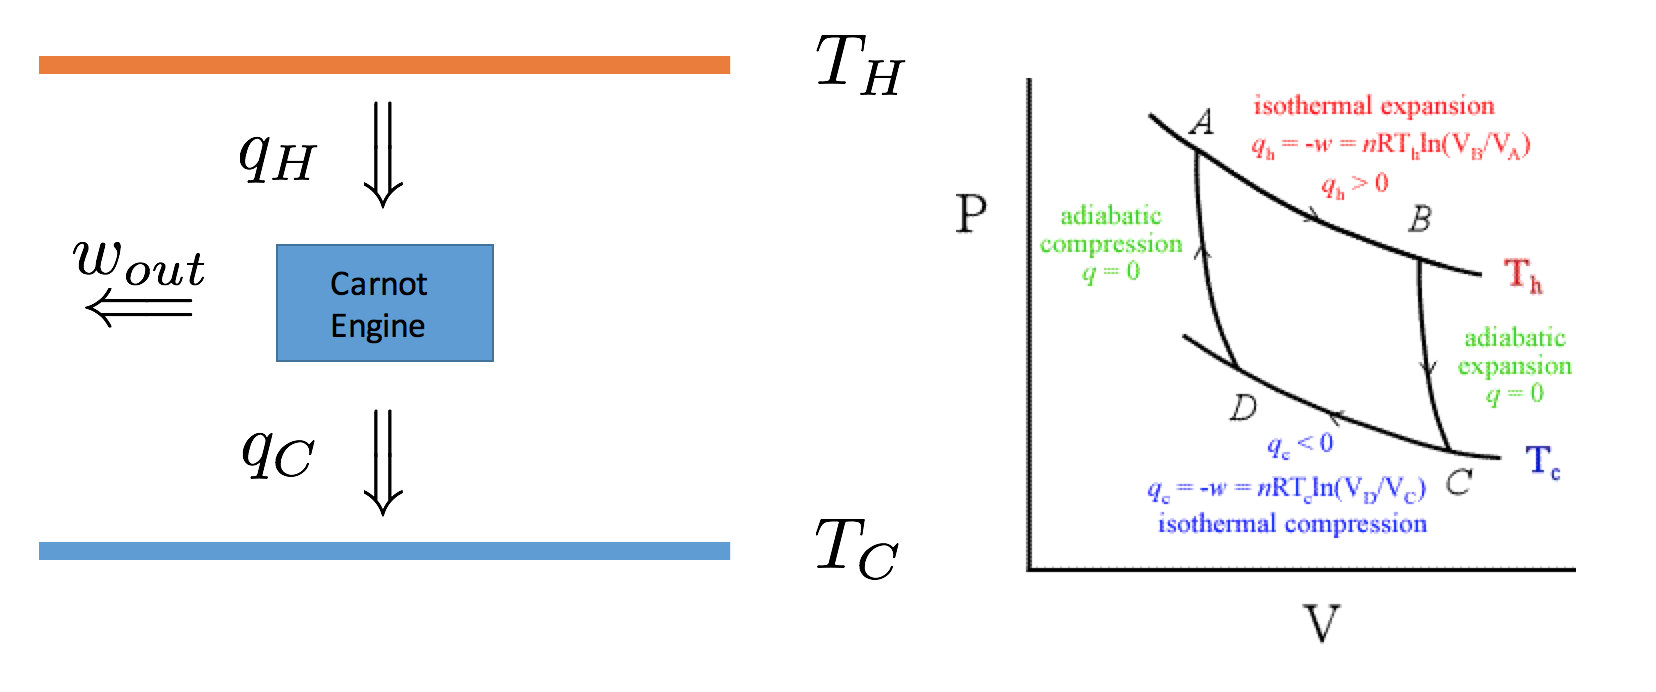
\includegraphics[width=17cm]{carnot.png}
    \caption{Carnot Cycle (Image taken from Quora).}
    \label{fig:carnot}
\end{figure}

\benum
    \item A $\rightarrow$ B is an isothermal expansion at T$_H$. 
    \item B $\rightarrow$ C is an adiabatic expansion, q = 0. 
    \item C $\rightarrow$ D is an isothermal compression at T$_C$. 
    \item D $\rightarrow$ A is an adiabatic compression, q = 0.     
\eenum

\subsection*{A $\rightarrow$ B; Reversible Isothermal Expansion at T$_H$}
Because this expansion is done isothermally with an ideal gas, the internal energy must be 0, so the first law states q = -W. 
The process is done reversibly, so we can substitute in our ideal gas law.
This step is occurring at the higher temperature, therefore this heat must be the heat at the higher temperature (q$_H$) in our generic engine diagram. 
\be
\begin{split}
W_{AB} &= -\int_A^B P_{ext}dV = -\int_A^B \frac{nRT_H}{V}dV = -nRT\ln\left(\frac{V_B}{V_A}\right) \\
q_{AB} &= q_H = nRT_H\ln\left(\frac{V_B}{V_A}\right) \\
\Delta S_{AB} &= \frac{q_{r}}{T} = \frac{q_H}{T_H} = nR\ln\left(\frac{V_B}{V_A}\right)
\end{split}
\ee
The sign of q should be positive during this step. The temperature at the beginning of the cycle is large, the heat therefore enters our engine and can be used to get some useful work out of the system. 

\subsection*{B $\rightarrow$ C; Reversible Adiabatic Expansion q = 0}
We are now doing a further expansion adiabatically, q$_{BC}$ = 0 by definition.
Therefore the temperature must change because of lack in heat transfer.  
This means the entropy change for this process is also 0, $\Delta$S$_{BC}$ = 0.

Because we are expanding we expect the temperature to decrease if no heat enters the system (the molecules have farther to travel so the average energy decreases). 
Because the process is done adiabatically we know that we can write the first law as U = W.
For an ideal gas (assume monoatomic) the equipartition theorem tells us that
\be
\begin{split}
    U(T) &= \frac{3}{2}kT = \frac{3}{2}nRT \\
    \Delta U_{BC}(T) &= \frac{3}{2}nR\Delta T = \frac{3}{2}nR(T_C-T_H)  \\
    W_{BC} &= \frac{3}{2}nR(T_C-T_H) 
\end{split}
\ee

By construction the cold temperature must be lower than the hot temperature, therefore the Internal Energy decreases during this step. 

\subsubsection*{C $\rightarrow$ D; Reversible Isothermal Compression at T$_C$}
To complete our cycle we must end up at the same initial state, therefore we need to compress our gas (a state is defined by the P,V, T coordinates in this system). 
We are not simply 'rewinding' however, because the heat and work will be unique, specifically we are working at the lower temperature now. 
So yes we are going to put work back into our system, but doing so at a lower temperature will give us a net profit of useful work from the engine.  

\be
\begin{split}
\Delta U_{CD} &= 0 \\
W_{CD} &= -nRT_C\ln\left(\frac{V_D}{V_C}\right) \\
q_{CD} &= q_C = nRT_C\ln\left(\frac{V_D}{V_C}\right) \\
\Delta S_{CD} &= \frac{q_C}{T_C} = nR\ln\left(\frac{V_D}{V_C}\right)
\end{split}
\ee

\subsection*{D $\rightarrow$ A; Reversible Adiabatic Compression q = 0}
Again from the same argument in the adiabatic expansion, the Entropy and heat are both 0
We can calculate the change in Internal Energy (and therefore work) using the equipartition theorem for an ideal gas. 
\be
\begin{split}
    q_{DA} &= 0 \\
    \Delta S_{DA} &= 0\\
    \Delta U_{DA} &= \frac{3}{2} nR(T_H-T_C)\\
    W_{DA} &= \frac{3}{2} nR(T_H-T_C)
    \end{split}
\ee

\subsection*{Cycle Analysis}
Internal Energy is a state function meaning any path we take will not effect the final result.
Consider each step in our process:
\be
\begin{split}
\Delta U_{cycle} &= U_{AB} + U_{BC} + U_{CD} + U_{DA} \\
& = 0 + \frac{3}{2}nR(T_C-T_H) + 0 + \frac{3}{2}nR(T_H-T_C) = 0
\end{split}
\ee
And as we expect, the Internal Energy only depends on the initial and final states for a process.
If we complete a cycle the initial and final state are the same and we get a $\Delta$ of 0. 

Now repeating the calculation for entropy we find:
\be
\begin{split}
\Delta S_{cycle} &= S_{AB} + S_{BC} + S_{CD} + S_{DA} \\
& =  nR\ln\left(\frac{V_B}{V_A}\right) + 0 +  nR\ln\left(\frac{V_D}{V_C}\right) + 0 \\
\Delta S_{cycle} &= nR\ln\left(\frac{V_BV_D}{V_AV_C}\right)
\end{split}
\ee

To simplify this last line we note that an adiabatic expansion/compression can be characterized by T$^\#$V = constant. 
So consider a ratio between our two temperatures during the adiabatic processes at both the beginning and end of the expansion/compression.
\be
\begin{split}
T(A)V(A) \propto T(D)V(D) &\implies \frac{T^{\frac{3}{2}}_H}{T^{\frac{3}{2}}_C} = \frac{V_D}{V_A}\\
T(B)V(B) \propto T(C)V(C) &\implies \frac{T^{\frac{3}{2}}_H}{T^{\frac{3}{2}}_C} = \frac{V_C}{V_B}\\ 
&\implies\\
\frac{V_D}{V_A} &= \frac{V_C}{V_B} \implies \frac{V_BV_D}{V_AV_C} = 1
\end{split}
\ee
And with this comparison we also shown that the Entropy of the entire cycle must be 0 (ln[1] = 0). 

Now consider the path functions:
\be
\begin{split}
    W_{cycle} &= -nRT_H\ln\frac{V_B}{V_A} + \frac{3}{2} nR(T_C-T_H) + -nRT_C\ln\frac{V_D}{V_C} + \frac{3}{2} nR(T_H-T_C) \\
    &= -nRT_H\ln\frac{V_B}{V_A} + -nRT_C\ln\frac{V_A}{V_B} \\
    W_{out}&= -nR\ln\frac{V_B}{V_A}(T_H-T_C)
\end{split}
\ee
We note that the total work is negative, this means our system DID work on the surroundings (we got useful work out of the engine). 
So the larger in magnitude we make this number the more we can get out of our engine. 

Let's now look at our heat, we know q$_H$ enters our system (positive value with our convention), and q$_c$ leaves our system to satisfy the Second Law (so this will be negative in our convention). 
We are going to use our relationship between the volumes from above to put everything in terms of A and B for the sake of comparison. 
\be
\begin{split}
    q_H &= q_{AB} = nRT_H \ln \left(\frac{V_B}{V_A}\right)\\
    q_C &= q_{CD} = nRT_C \ln \left(\frac{V_D}{V_C}\right) = -nRT_C \ln \left(\frac{V_B}{V_A}\right) 
\end{split}
\ee

If we now consider the First Law we know that 
\be
q_C = q_H + W_{out} \implies q_H = q_C + W_{out}
\ee
And if you plug in our expressions from above and do the algebra this relationship holds true. 

Finally if we consider our Second Law, we know the Entropy change of the cycle is 0.
We define the Entropy of the environment as simply the heat that enters it divided by the temperature (what heat enters/leaves each reservoir). 
\be
\Delta S_{univ} = \Delta S_{cycle} + \Delta S_{H,res} + \Delta S_{C,res} = 0 + \frac{-q_H}{T_H} + \frac{q_C}{T_C} = -nR\ln\frac{V_B}{V_A} + nR\ln\frac{V_B}{V_A} = 0
\ee
And again as expected for a reversible processes, we did not change the Entropy of the universe over the entire cycle. 

\end{document}